\section{Kan complexes}

lecture 19.11

For references for this section see \cite[Section I.3]{GoerSimp1999} \& \cite[Section 1.2.5]{kerodon}.

The aim of this chapter is to introduce a calss of simplicaial sets that behave simultaneously as nerves of groupoids and singular sets of spaces.

\begin{defi}
    Let $n \geq 1$ and $ 0 \leq k \leq n$.
    The $k$-th horn $\Lambda_k^n \subseteq \Delta^n$ is the simplicial subset generated by $\{ d^i \colon [n-1] \to [n] \mid 0 \leq i \leq n ; i \neq n \} = \Delta ( n-1,n) = (\Delta^n)_{n-1}$ , or equivalently $\Lambda_k^n = \colim_{\emptyset \neq k \in I \subsetneq [n]}\Delta^I$ where $\Delta^I \cong \Delta^{\lvert I \rvert -1}$.
\end{defi}

\begin{rmk}
    We will sometimes refer to $\Lambda_k^n$ as the $n$-horn at position $k$.     
\end{rmk}

\begin{exmp}
    Let us give a list for the horns up to dimension 3
    \begin{itemize}
        \item 
        For $ n = 1 $ we have the two horns $\Lambda_0^1 =0 $ and $\Lambda_1^1=1$.
        \item 
        For $ n = 2 $ we have the following 3 horns, given here with their embedding into the standard 2-simplex
        \[
        \Lambda_0^2 \colon 
        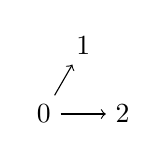
\begin{tikzpicture}[baseline={(0,0.3)}]
            \node (A) at (0,0.866) {$1$};
            \node (B) at (-0.5,0) {$0$};
            \node (C) at (0.5,0) {$2$};
            \draw [->] (B) -- (A);
            \draw [->] (B) -- (C);
        \end{tikzpicture}
        \hookrightarrow
        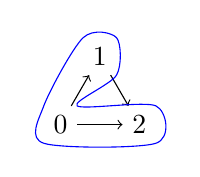
\begin{tikzpicture}[baseline={(0,0.3)}]
            \node (A) at (0,0.866) {$1$};
            \node (B) at (-0.5,0) {$0$};
            \node (C) at (0.5,0) {$2$};
            \draw [->] (A) -- (C);
            \draw [->] (B) -- (A);
            \draw [->] (B) -- (C);
            \draw [blue] plot [smooth cycle] coordinates {(A.north west)     (A.north east) (A.south east) (B.north east) (C.north east) (C.south east) (B.south west) (B.north west) };
        \end{tikzpicture}
        \]
        \[
        \Lambda_1^2 \colon 
        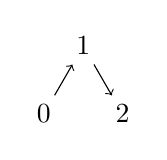
\begin{tikzpicture}[baseline={(0,0.3)}]
            \node (A) at (0,0.866) {$1$};
            \node (B) at (-0.5,0) {$0$};
            \node (C) at (0.5,0) {$2$};
            \draw [->] (B) -- (A);
            \draw [->] (A) -- (C);
        \end{tikzpicture}
        \hookrightarrow
        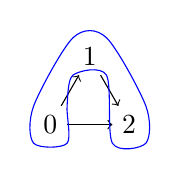
\begin{tikzpicture}[baseline={(0,0.3)}]
            \node (A) at (0,0.866) {$1$};
            \node (B) at (-0.5,0) {$0$};
            \node (C) at (0.5,0) {$2$};
            \draw [->] (A) -- (C);
            \draw [->] (B) -- (A);
            \draw [->] (B) -- (C);
            \draw [blue] plot [smooth cycle] coordinates {(A.north west) 
            (A.north east) (C.north east) (C.south east) (C.south west) (A.south east) (A.south west) (B.north east) (B.south east) (B.south west) (B.north west) };
        \end{tikzpicture}
        \]
        \[
        \Lambda_2^2 \colon 
        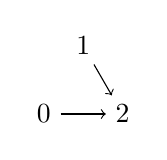
\begin{tikzpicture}[baseline={(0,0.3)}]
            \node (A) at (0,0.866) {$1$};
            \node (B) at (-0.5,0) {$0$};
            \node (C) at (0.5,0) {$2$};
            \draw [->] (A) -- (C);
            \draw [->] (B) -- (C);
        \end{tikzpicture}
        \hookrightarrow
        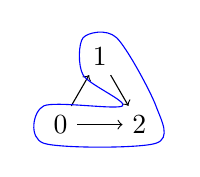
\begin{tikzpicture}[baseline={(0,0.3)}]
            \node (A) at (0,0.866) {$1$};
            \node (B) at (-0.5,0) {$0$};
            \node (C) at (0.5,0) {$2$};
            \draw [->] (A) -- (C);
            \draw [->] (B) -- (A);
            \draw [->] (B) -- (C);
            \draw [blue] plot [smooth cycle] coordinates {(A.south west) (A.north west) (A.north east) (C.north east) (C.south east) (B.south west) (B.north west) (C.north west) };
        \end{tikzpicture}
        \]
    \end{itemize}
\end{exmp}

\begin{rmk}
    The horn $\Lambda_k^n \subseteq \Delta^n$ enjoys the following universal property:
    For $X \in \SetD$ the map 
    \[
    \begin{tikzcd}
        \Hom_{\SetD}(\Lambda_k^n,X)
        \arrow[r, hook]
        &
        \prod_{\substack{0\leq i \leq \\ i \neq k}}
        \Hom_{\SetD}(\Delta^{n-1},X)
        \\
        \sigma 
        \arrow[r, mapsto]
        &
        (\sigma \circ d^i)_{\substack{0 \leq i \leq n \\ i \neq k}}
    \end{tikzcd}
    \]
    is injective, with image the subset of tuples $(\sigma_0,\sigma_1,\dotsc,\sigma_{k-1},\cdot, \sigma_{k+1}, \dotsc, \sigma_n) \in (X_{n-1})^n$ such that for all $ 0 \leq i < j \leq n$, $i \neq k$ $d_(\sigma_j)=d_{j-1}(\sigma_i)$ with $I = [n] \setminus \{i\}$ and $J=[n]\setminus \{j\}$ the following diagrams commute
    \[
    \begin{tikzcd}
    	& {\Delta^{I \cap J}} \\
    	{\Delta^I} && {\Delta^J} \\
    	& {\Lambda_k^n}
    	\arrow[hook', from=1-2, to=2-1]
    	\arrow[hook, from=1-2, to=2-3]
    	\arrow[from=2-1, to=3-2]
    	\arrow[from=2-3, to=3-2]
    \end{tikzcd}
    \qquad
    \begin{tikzcd}
        & \Delta^{n-2} \\
        \Delta^{n-1} && \Delta^{n-1} \\
        & \Delta^n
        \arrow[from=1-2, to=2-1, "d^{j-1}"']
        \arrow[from=1-2, to=2-3, "d^{i}"]
        \arrow[from=2-1, to=3-2, "d^{i}"']
        \arrow[from=2-3, to=3-2, "d^{j}"]
    \end{tikzcd}
    \]
\end{rmk}

\begin{defi}
    Let $X \in \SetD $, $X$ is a \underline{Kan complex} ($=\infty$-groupoid) if for all $n\geq 1$ and all morphisms $\sigma\colon \Lambda_k^n \to X$ we have the following diagram:
    \[
    \begin{tikzcd}
        \Lambda_k^n
        \arrow[r, "\sigma"]
        \arrow[d, hook, "\can"']
        &
        X
        \\
        \Delta^n
        \arrow[ur, dashed, "\exists \widehat{\sigma}"']
    \end{tikzcd}
    \]
\end{defi}

\begin{rmk}
        Notice that the morphism $\widehat{\sigma}$ need not be unique.
\end{rmk}

Recall the following adjunctions
\[
\begin{tikzcd}
        \Gpd
        \arrow[r, bend left, "j",""{name=A, above}]
        &
        \Cat
        \arrow[l, bend left ,"L" pos=0.45,""{name=B, above}]
        \arrow[from=A, to=B, symbol=\dashv]
        \arrow[r, bend left, "N",""{name=C, above}]
        &
        \Set_{\Delta}       
        \arrow[l, bend left ,"\tau" pos=0.45,""{name=D, above}]
        \arrow[from=C, to=D, symbol=\dashv]
        \arrow[r, bend left ,"\lvert\cdot\rvert" pos=0.45,""{name=E, above}]
        &
        \Top      
        \arrow[l, bend left, "\Sing",""{name=F, above}]
        \arrow[from=E, to=F, symbol=\dashv]
\end{tikzcd}
\]

\begin{prop}
    Let $X \in \Top$.
    Then $\Sing(X)$ is a Kan complex.
\end{prop}

\begin{proof}
    For all $n \geq 1$ and $0 \leq k \leq n$ we want the following diagram:
    \[
    \begin{tikzcd}
        \Lambda_k^n 
        \arrow[d, hook, "\iota"']
        \arrow[r, "\sigma"]
        &
        \Sing(X)
        \\
        \Delta^n
        \arrow[ru, dashed ,"\exists \Tilde{\sigma}"']
    \end{tikzcd}
    \]
    Now after applying the geometric realization functor $\lvert \cdot\rvert$ to the above diagram, we obtain a diagram
    \[
    \begin{tikzcd}
        \lvert \Lambda_k^n \rvert
        \arrow[d, hook, shift right, "\lvert \iota \rvert"']
        \arrow[r, "\overline{\sigma}"]
        &
        X
        \\
        \lvert \Delta^n \rvert
        \arrow[ru, "\alpha= \Bar{\sigma} \circ r"']
        \arrow[u, shift right, "\exists r"']
    \end{tikzcd}
    \]
    where $r$ is a continuous retraction of $\Delta^n$ onto $\lvert \Lambda_k^n \rvert$.
    Then we apply the adjunction to the following composition
    \[
    \lvert \Lambda_k^n\rvert 
    \xrightarrow{\lvert \iota \rvert} 
    \lvert \Delta^n\rvert
    \xrightarrow{\alpha}
    X = \lvert \Lambda_k^n\rvert 
    \xrightarrow{\lvert \sigma \rvert}
    X
    \]
    to obtain 
    \[
    \Lambda_k^n
    \xrightarrow{\iota}
    \Delta^n
    \xrightarrow{\overline{\alpha}}
    \Sing(X) = \Lambda_k^n
    \xrightarrow{\overline{\overline{\sigma}}=\sigma}
    \Sing(X)
    \]
    which then gives the desired horn extension:
    \[
    \begin{tikzcd}
        \Lambda_k^n 
        \arrow[d, "\iota"']
        \arrow[r, "\sigma"]
        &
        \Sing(X)
        \\
        \Delta^n
        \arrow[ru, "\overline{\alpha}\eqqcolon \Tilde{\sigma}"']
    \end{tikzcd}
    \]
\end{proof}

\begin{defi}
    Let $X \in \SetD$, it is called an \underline{inner Kan complex} ($=\infty$-category) if for all $n\geq 2$ and $0 < k < n $ we have the following diagram:
    \[
    \begin{tikzcd}
        \Lambda_k^n
        \arrow[r, "\sigma"]
        \arrow[d, hook, "\can"']
        &
        X
        \\
        \Delta^n
        \arrow[ur, dashed, "\exists \widehat{\sigma}"']
    \end{tikzcd}
    \]
\end{defi}

\begin{rmk}
    Let $n \geq 0$ and 
    $\Delta_{\leq n} \coloneqq \{ [m] \in \Delta \mid 0 \leq m \leq n\}\xhookrightarrow{\iota} \Delta$ as well as $\tru_n = \iota^*$. 
    We have the following adjunction
    \[
    \begin{tikzcd}
        \SetD
        &
        \Set_{\Delta_{\leq n}}= \Fun(\Delta^{\op}_{\leq n} , \Set)
        \arrow[from=1-1, to=1-2, "\tru_n"]
        \arrow[from=1-2, to=1-1, bend left, hook', "\cosk_n" pos=0.45]
        \arrow[from=1-2, to=1-1, bend right, hook,"\sk_n"']
    \end{tikzcd}
    \]
    and call $X \in \SetD$ n-coskeletal if the following equivalent conditions hold:
    \begin{enumerate}
        \item 
        $X \in \Ima(\cosk_n)$
        \item 
        $X \isomorphism \cosk_n(\tru_n)$
        \item 
        $\forall Y \in \SetD: \Hom_{\SetD}(Y,X) \isomorphism \Hom_{\Set_{\Delta_{\leq n}}}(\tru_n Y, \tru_n X)$
    \end{enumerate}
    Also note that for $\mathcal{C} \in \Cat$ we have that $N(\mathcal{C)} \in \SetD$ is 2-coskeletal.
\end{rmk}

\begin{prop}
    Let $\mathcal{C} \in \Cat$. The nerve of $\mathcal{C}$ is an inner Kan complex.
\end{prop}

\begin{proof}
    Let $n \geq 2$ and $0 < k <n$, consider the horn extension diagram
    \[
    \begin{tikzcd}
        \Lambda_k^n
        \arrow[r, "\sigma"]
        \arrow[d, hook]
        &
        N(\mathcal{C})
        \\
        \Delta^n
        \arrow[ur, dashed, "\exists \widehat{\sigma} ?"']
    \end{tikzcd}
    \]
    By coskeletality of $N(\mathcal{C})$ it is enough to solve the 2-truncated extension
    \[
    \begin{tikzcd}
        \tru_n(\Lambda_k^n)
        &
        \tru_2(N(\mathcal{C}))
        \\
        \tru_n(\Delta^n)
        \arrow[from=1-1, to=1-2, "\tru_2 \sigma"]
        \arrow[from=1-1, to=2-1, "\tru_2 (\iota)"]
        \arrow[from=2-1, to=1-2, "\tru_2 \circ \exists \Tilde{\sigma}?"']
    \end{tikzcd}    
    \]
    For $n \geq 4$ we have that $\tru_2(\Lambda_k^n)=\tru_2(\Delta^n)$ and hence the problem is trivial in that case.
    For $n=2$ we have that $0 < k < 2$, thus $k=1$, so we consider the horn at 1 and the corresponding horn extension problem
    \[
    \begin{tikzcd}
        &
        1
        &
        \\
        0
        &&
        2
        \arrow[from=2-1, to=1-2]
        \arrow[from=1-2, to=2-3]
    \end{tikzcd}
    \qquad
    \begin{tikzcd}
        \Lambda_1^2
        &
        N(\mathcal{C})
        \\
        \Delta^n
        \arrow[from=1-1, to=1-2, "\sigma"]
        \arrow[from=1-1, to=2-1]
        \arrow[from=2-1, to=1-2,dashed,"\Tilde{\sigma}"']
    \end{tikzcd}
    \]
    So $\sigma$ is explicitely given as 
    \[
    \begin{tikzcd}
        &
        X_1
        &
        \\
        X_0
        &&
        X_2
        \arrow[from=2-1, to=1-2,"\sigma_{10}"]
        \arrow[from=1-2, to=2-3,"\sigma_{21}"]
    \end{tikzcd}
    \] 
    so we can choose $\sigma_{21}\circ\sigma_{10}$ to complete the horn to a full simplex giving the desired horn extension.
    For $n=3$ we have the $k=1,2$, we are going to consider the case $k=1$ explicitly. 
    We get the following simplex diagramm
    \[
        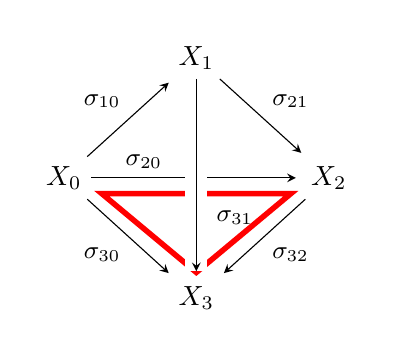
\begin{tikzpicture}[>=stealth,->,shorten >=2pt,looseness=.5,auto]
            \matrix[anchor=center, column sep=1cm, row sep=1cm] at (0,0)
            {
                                & \node(X_1) {$X_1$};   &                 \\
             \node(X_0) {$X_0$};     &                  & \node(X_2) {$X_2$};  \\
                                & \node(X_3) {$X_3$};   &                 \\
            };
            \draw[line width=2pt,color=red] (-1.2,-0.2) -- (1.2,-0.2) -- (0,-1.2) -- cycle;
            \begin{scope}[every node/.style={font=\small\itshape}]
                \draw (X_1) -- node [midway] {$\sigma_{21}$} (X_2);
                \draw (X_0) -- node [midway] {$\sigma_{10}$} (X_1);
                \draw (X_0) -- node [midway, swap] {$\sigma_{30}$}(X_3);
                \draw (X_0) -- node [near start] {$\sigma_{20}$}(X_2);
                \draw [-,line width=8pt,draw=white]
                (X_1) -- node [pos=0.7] {$\sigma_{31}$} (X_3);
                \draw (X_1) -- (X_3);
                \draw (X_2) -- node [midway] {$\sigma_{32}$} (X_3);
            \end{scope}
        \end{tikzpicture}              
    \]
    where the red triangle is not commuting a priori.
    The simplex gives the following identities
    \[
    \sigma_{30} = \sigma_{32} \circ \sigma_{20} \iff \sigma_{30} = \sigma_{32} \circ (\sigma_{21} \circ \sigma_{10}) = (\sigma_{32} \circ \sigma_{21}) \circ \sigma_{10} = \sigma_{31} \circ \sigma_{10} = \sigma_{30}
    \]
    which yields the commutativity of the bottom simplex.
\end{proof}

\begin{prop}
    Let $\mathcal{C} \in \Cat $. Then the following are equivalent:
    \begin{enumerate}
        \item 
        $\mathcal{C}$ is a groupoid,
        \item 
        $N(\mathcal{C})$ is a Kan complex.
    \end{enumerate}
\end{prop}

\begin{proof}
    "$2) \implies 1)$" 
    Let $f\colon X \to Y$ be a morphism in $\mathcal{C}$. 
    The horns 
    \[
    \begin{tikzcd}
        &
        Y
        \arrow[rd, dashed, "\exists g"]
        &\\
        X
        \arrow[ru, "f"]
        \arrow[rr,"1_X"']
        &
        &
        X
    \end{tikzcd}
    \qquad
    \begin{tikzcd}
        &
        X
        \arrow[rd, "f"]
        &\\
        Y
        \arrow[ru, dashed, "\exists h"]
        \arrow[rr,"1_Y"']
        &
        &
        Y
    \end{tikzcd}
    \]
    extend to 2-simplices of $N(\mathcal{C})$ since $N(\mathcal{C})$ is a Kan complex.
    So we get that $gf=\id_X$ and $fh=\id_Y$.
    Thus $\mathcal{C}$ is a groupoid.
    "$1) \implies 2)$"
    We already know that $N(\mathcal{C})$ is an inner Kan complex.
    "$1) \implies 2)$"
    We already know that $N(\mathcal{C})$ is an inner Kan complex.
    It is enough to consider the cases $n=2$, $k=0,2$ and $n=3$ $k=0,3$ by 2-coskeletality of $N(\mathcal{C})$.
    For $n=2$ and $k=0$ we have that the diagram 
    \[
    \begin{tikzcd}
        &X_1&\\
        X_0
        \arrow[ru, "\sigma_{10}"]
        \arrow[rr, "\sigma_{20}"']
        &&
        X_2
    \end{tikzcd}
    \]
    in $\mathcal{C}$, extends to 
    \[
    \begin{tikzcd}
        &X_1
        \arrow[rd, dashed, "\sigma_{20} \circ \sigma_{10}^{-1}"]
        &\\
        X_0
        \arrow[ru, "\sigma_{10}"]
        \arrow[rr, "\sigma_{20}"']
        &&
        X_2
    \end{tikzcd}
    \]
    where $\sigma_{20} \circ \sigma_{10}^{-1}$ exists since $\mathcal{C}$ is a groupoid.
    The case for $k=2$ is done analogously.
    For $n=3$ and $k=2$, consider the following 2-simplex
    \[
        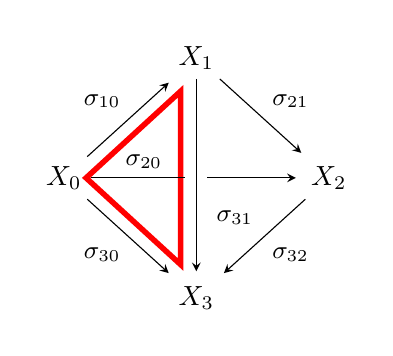
\begin{tikzpicture}[>=stealth,->,shorten >=2pt,looseness=.5,auto]
            \matrix[anchor=center, column sep=1cm, row sep=1cm] at (0,0)
            {
                                & \node(X_1) {$X_1$};   &                 \\
             \node(X_0) {$X_0$};     &                  & \node(X_2) {$X_2$};  \\
                                & \node(X_3) {$X_3$};   &                 \\
            };
            \draw[line width=2pt,color=red] (-0.2,1.1) -- (-0.2,-1.1) -- (-1.4, 0) -- cycle;
            \begin{scope}[every node/.style={font=\small\itshape}]
                \draw (X_1) -- node [midway] {$\sigma_{21}$} (X_2);
                \draw (X_0) -- node [midway] {$\sigma_{10}$} (X_1);
                \draw (X_0) -- node [midway, swap] {$\sigma_{30}$}(X_3);
                \draw (X_0) -- node [near start] {$\sigma_{20}$}(X_2);
                \draw [-,line width=8pt,draw=white]
                (X_1) -- node [pos=0.7] {$\sigma_{31}$} (X_3);
                \draw (X_1) -- (X_3);
                \draw (X_2) -- node [midway] {$\sigma_{32}$} (X_3);
            \end{scope}
        \end{tikzpicture}              
    \]
    which gives the following chain of identities:
    \[
    \sigma_{31} \circ \sigma_{10}= \sigma_{32} \circ \sigma_{21} \circ \sigma_{10} = \sigma_{32} \circ \sigma_{20} = \sigma_{30}
    \]
\end{proof}

Lecture 21.11

\begin{exmp}
    \begin{enumerate}
        \item 
        For all $X \in \Top$, $\Sing(X) \in \SetD$ is a Kan complex.
        \item 
        For all $\mathcal{C} \in \Cat$, $N(\mathcal{C})$ is an inner Kan complex.
        \item 
        $N(\mathcal{C)}$ is a Kan complex if and only if $\mathcal{C}$ is a groupoid.
        \item 
        For all $n\geq 0$, $\Delta^n=N([n])$ is an inner Kan complex and furthermore $\Delta^n$ is a Kan complex if and only if $n=0$.
        \item 
        If $M$ is a monoid then $N(BM)$ is an inner Kan complex and furthermore $N(BM)$ is a Kan complex if and only if $M$
    \end{enumerate}
\end{exmp}

\begin{defi}
    The category of simplicial groups is $\Fun(\Delta^{\op},\Grp)$. 
    Thus $X \in \Fun(\Delta^{\op},\Grp)$ consists of the following data:
    \begin{itemize}
        \item 
        For all $n\geq 0$ a group $X_n$ with a neutral element $e_n\in X_n$.
        \item 
        For all $0 \leq i \leq n$
        \begin{tabular}{c}
              $d_i\colon X_n \to X_{n-1}$ face map \\
              $s_i\colon X_n \to X_{n+1}$ degeneracy map,
        \end{tabular}
        satisfy the simplicial identities and are group homomorphisms.
    \end{itemize}
\end{defi}

\begin{prop}
    Let $X$ be a simplicial group. 
    Then the underlying simplicial set of $X$ is a Kan complex.
\end{prop}

\begin{proof}
    The case $n=1$ is trivial.
    We illustrate the argument for $n=2$ and $k=1$.
    Suppose given a horn 
    \[
    \begin{tikzcd}
        &
        x_1
        \arrow[rd, "x_{21}"]
        & \\
        x_0
        \arrow[ru, "x_{10}"]
        \arrow[rr, dashed, "\exists w"']
        &&
        x_2
    \end{tikzcd}
    \]
    Form the degenerate $2$-simplex $y \eqqcolon s_0(x_{21})$
    \[
    \begin{tikzcd}
        x_1
        \arrow[rd, "x_{21}"]
        &
        \\
        x_1
        \arrow[u, dashed, "1_{x_1}"]
        \arrow[r, "x_{21}"']
        &
        x_2
    \end{tikzcd}
    \]
    Let $z \coloneqq d_2(y) = 1_{X_1} \in X_1$.
    Consider now $s_1(x_{10}z^{-1})=s_1(x_{10}d_2(y)^{-1})=d_2(y^{-1})$.
    \[
    s_1(x_{10}z^{-1}):
    \begin{tikzcd}
        &
        x_1x_1^{-1}=e_0
        \arrow[rd, "1_{e_0}=s_0(e_0)=e_1"]
        &
        \\
        x_0x_1
        \arrow[ru, "x_{10}1_{x_1}^{-1}"]
        \arrow[rr, "x_{10}1_{x_1}^{-1}"']
        &&
        x_1x_1^{-1}=e_0
    \end{tikzcd}
    \]
    Let $w \coloneqq s_1(x_{10}z^{-1})y\in x_2$ and we get the chain of equalities
    \[
        d_0(w)=d_0((s_1(x_{10}z^{-1}))y)=d_0(s_1(x_{10}z^{-1}))d_0(y)=e_1x_{21}=x_{21}
    \]
    as well as 
    \[
    d_2(w)=d_2(s_1(x_0z^{-1}))d_2(y)=(x_{10}1_{x_1}^{-1})1_{x_1}=x_{10}e_1=x_{10}
    \]
    For the general case, consider a horn 
    \[
    (x_0,x_1,\dotsc, x_{k-1},\bullet,x_{k+1},\dotsc,x_n) 
    \]
    in $X$. Where $x_i \in X_{n-1}$ and $ d_i(x_j)=d_{j-1}(x_i)$ for $i<j$ and $i,j \neq k$.
    Suppose that there exists a $y \in X_n$ such that for all $ 0 \leq i < k$ and for all $l \leq i \leq n$.
    Then $w \coloneqq s_{l-2}(x_{l-1}\dotsm d_{l-1}(y)^{-1})y$ satisfies $d_i(w)=x_i$ for all $0 \leq i <k$ and all $l-1\leq i \leq n$.
\end{proof}

Recall the Dold-Kan correspondence.
\[
\begin{tikzcd}
    \tau \colon \Ab_{\Delta}
    \arrow[d, "\text{forgetfull}"']
    \arrow[r,"\sim"]
    &
    \Ch_{\leq} (\Ab)\colon Dk
    \arrow[l]
    \arrow[d, hook]
    &
    \\
    \SetD
    &
    \Ch(\Ab)
    \arrow[r,"\gamma"]
    &
    D(\Ab)
\end{tikzcd}
\]

\begin{prop}
    Let $X$ be a Kan complex ($X \in \SetD$).
    Then $x,y \in X_0$ satisfy $[x]=[y]$ in $\pi_0(X)$ if and only if there exists a $\sigma \in X_1$ such that $d_0(\sigma)=y$ and $d_1(\sigma)=x$.
\end{prop}

\begin{proof}
    At first, when there is a $\sigma$ that relates $X$ to $Y$ we can complete this to 1-simplex
    \[
    \begin{tikzcd}
        &
        Y
        \ar[rd, "d_0(\tau)"]
        &
        \\
        X
        \ar[ru,"\sigma"]
        \ar[rr,"1_X"']
        &&
        X
    \end{tikzcd}
    \]
    and obtain $d_0(\tau)$ that relates $Y$ to $X$.
    Also if $X$ relates to $Y$ and $Y$ relates to $Z$, we obtain a $2$-simplex
    \[
    \begin{tikzcd}
        &
        Y
        \ar[rd, "\tau"]
        &
        \\
        X
        \ar[ru,"\sigma"]
        \ar[rr,"d_1(\alpha)"']
        &&
        Z
    \end{tikzcd}
    \]
    where $d_1(\alpha)$ relates $X$ to $Z$.
\end{proof}

\subsection{Exercises}

\begin{Exercise}
    \begin{enumerate}[label=(\alph*)]
        
        \item 
        Show that for $ n \in \mathbb{N}_0 $ we have $ \bold{sk}_n ( \Delta^{n+1} ) \cong \partial \Delta^{n+1}$.
    
        \item 
        Show that for every horn $ \Lambda_k^m $ we have that 
        \[
            \bold{sk_n} ( \Lambda_k^m ) \cong 
            \begin{cases}
                \Lambda_k^m &\text{ if } m \leq n+1
                \\
                \bold{sk}_n ( \Delta^m ) &\text{ if } m > n+1
            \end{cases}
        \]
        for $ 0 \leq k \leq m \in \mathbb{ N }_+$.
    
        \item 
        Show that for a Kan comlex $ K $ and any $ n \in \mathbb{N}_0 $, the $ n $-coskeleton $\bold{cosk}_n ( K ) $ is a Kan complex.
        
    \end{enumerate}
\end{Exercise}

\begin{Exercise}
    \begin{enumerate}[label=(\alph*)]
        \item 
        Show that the class of Kan complexes and the class of inner Kan complexes are closed under set indeced products.
    
        \item 
        Show that a set indexed product of connected Kan complexes is connected.
    
        \item 
        Give an example that an infinite product of connected inner Kan complexes is not necessarily connected. 
        ( Recall that the nerve of a category is an inner Kan complex.)
    \end{enumerate}
\end{Exercise}